\chapter{Background}
\label{chap:background}

\section{Introduction}

This chapter provides a short and non-exhaustive overview of the theory and techniques used in this thesis.

First Section~\ref{subsec:background-terminology} defines the terminology. Then Section~\ref{subsec:background-statistics} describes the statistical tools and methodologies used in this thesis. This is followed by Section~\ref{subsec:background-machine-learning} providing an overview of the machine learning techniques used in this thesis. Section~\ref{subsec:background-gpgpu} provides an overview of GPGPU programming. Finally Section~\ref{subsec:background-summary} concludes.

\todo{This entire chapter has yet to be written. All current text is placeholder.}

\section{Terminology}
\label{subsec:background-terminology}

\emph{machine learning}

\emph{deep learning}

\emph{feature space}

\emph{supervised learning}

\emph{unsupervised learning}


\section{Evaluation Techniques}
\label{subsec:background-statistics}

\subsection{Principal Component Analysis}


\section{Machine Learning}
\label{subsec:background-machine-learning}

\subsection{Decision Trees}

\subsection{Deep Learning}

\subsection{Recurrent Neural Networks}

A recurrent neural network (RNN) consists of hidden states \textbf{h} an an optional output \textbf{y}. It operates on a variable-length sequence, $\bm{x} = \left( x_1, x_2, \ldots, x_T \right)$. At each step $t \in T$, the hideen state $h_{<t>}$ of the RNN is updated by:

\[ h_{<t>} = f\left( h_{<t-1>}, x_t \right) \]

where $f$ is a non-linear activation function. An RNN can learn a probabilty distribution over a sequence of tokens to predict the next token. Therefore, at each timestep $t$, the output from the RNN is a conditional distribution $p\left( x_t | x_1, \ldots, x_{t-1} \right)$.

% De Boom, C., Dhoedt, B., & Demeester, T. (2018). Character-level Recurrent Neural Networks in Practice: Comparing Training and Sampling Schemes. ArXiv:1801.00632.
\todo[inline]{RNN evaluation~\cite{DeBoom2018}.}

\subsubsection{Long Short-Term Memory}

LSTM variants review~\cite{Greff2015}.

$\bm{x}^t$ is the input vector at time $t$; $\bm{W}$ are input weight matrices; $\bm{R}$ are recurrent weight matrices; $\bm{p}$ are peephole weight vectors; $\bm{b}$ are bias vectors; functions $g$, $h$, and $\sigma$ are point-wise nonlinear activation functions.

block input:
\[ \bm{z}^{t} = g \left( \bm{W}_z \bm{x}^t + \bm{R}_z \bm{y}^{t - 1} + \bm{b}_z \right) \]

input gate:
\[ \bm{i}^{t} = \sigma \left( \bm{W}_i \bm{x}^t + \bm{R}_i \bm{y}^{t-1} + \bm{p}_i \odot c^{t-1} + \bm{b}_i \right) \]

forget gate:
\[ \bm{f}^{t} = \sigma \left( \bm{W}_f \bm{x}^t + \bm{R}_f \bm{y}^{t-1} + \bm{p}_f \odot c^{t-1} + \bm{b}_f \right) \]

cell state:
\[ \bm{c}^t = \bm{i}^t \odot \bm{z}^t + \bm{f}^t \odot \bm{c}^{t-1} \]

output gate:
\[ \bm{o}^{t} = \sigma \left( \bm{W}_i \bm{x}^t + \bm{R}_o \bm{y}^{t - 1} + \bm{p}_o \odot c^{t-1} + \bm{b}_o \right) \]

block output:
\[ \bm{y}^t = \bm{o}^t \odot h(\bm{c}^t) \]

Number of params = \todo[inline]{\ldots}


% TODO: \subsection{Generative Adversarial Networks}

The Generative Adversarial Network (GAN) is a means to estimate a generative model~\cite{Goodfellow2014}. It uses an adversarial process in which two models are simultaneously trained: a generator model $G$ that captures the data distribution, and a discriminative model $D$ that estimates the probability that a sample came from the training data rather than $G$. The training procedure for $G$ is to maximise the probability of $D$ making a mistake.

If both models are neural networks: learn a generator's distribution $p_g$ over data $\bm{x}$. Define a prior on input noise variables $p_z(\bm{z})$. Generator $G(\bm{z}; \Theta_g)$, using parameters $\Theta_g$. Discriminator $D(\bm{x}; \Theta_d)$ outputs a scalar, the probability that $\bm{x}$ came from the data rather than $p_g$.

Simultaneously train $D$ to maximise the probability of assigning the correct label to both training examples and samples from $G$, and train $G$ to minimise $\log (1 - D(G(\bm{z})))$. $D$ and $G$ play the two-player minimax game with value function $V(G, D)$:

\[ \min_G \max_D V(D, G) = \mathbb{E}_{\bm{x} \sim  p_{data}(\bm{x})} [ \log D(\bm{x}) ] + \mathbb{E}_{\bm{z} \sim p_z(\bm{z})} [ \log (1 - D(G(\bm{z}))) ] \]

Challenge: there may not be sufficient gradient for $G$ to learn well. Early in learning, when $G$ is poor, $D$ can reject samples with high confidence because they are clearly different from the training data.


\section{GPGPU Programming}
\label{subsec:background-gpgpu}

General purpose programming with graphics hardware is a nascent field, but has shown to enable massive data parallel throughput by re-purposing the hardware traditionally dedicated to the rendering of 3D graphics for generic computation. This was enabled by hardware support for programmable shaders replacing the fixed function graphics pipeline, and support for floating point operations in 2001. \citeauthor{Owens2006} provide a review of the first five years of general purpose computation on graphics hardware in~\cite{Owens2006}.

In the ensuing progress towards increasingly programmable graphics hardware, two dominant programming models have emerged: CUDA and OpenCL, which both abstract the graphics primitives of GPU hardware and provide a platform for GPGPU programming. CUDA is a language developed by NVIDIA for programming their GPUs using a proprietary SDK and API~\cite{Nvidia2007}, while OpenCL is a vendor-independent open standard based on a subset of the ISO C99 programming language, with implementations for devices from most major GPU manufactures~\cite{Stone2010}. Quantitative evaluations of the performance of CUDA and OpenCL programs suggest that performance is comparable between the two systems, although the wider range of target architectures for OpenCL means that appropriate optimisations must be made by hand or by the compiler~\cite{Komatsu2010,Karimi2010}.


\subsection{The OpenCL Programming Model}

OpenCL is a parallel programming framework which targets CPUs, GPUs, and other parallel processors such as Field-Programmable Gate Arrays. It provides a set of APIs and a language (based on an extended subset of C) for controlling heterogeneous \emph{compute devices} from a central host. Programs written for these devices are called \emph{kernels}, and are compiled by platform-specific tool chains. At runtime, an OpenCL \emph{platform} is selected and a \emph{context} object is created which exposes access to each supported compute device through \emph{command queues}. When a kernel is executed, each unit of computation is referred to as a \emph{work-item}, and these work-items are grouped into \emph{work-groups}. The sum of all work-group dimensions defines the \emph{global size}. For GPUs, work-groups execute on the Single Instruction Multiple Data (SIMD) processing units in lockstep. This is very different from the behaviour of traditional CPUs, and can cause severe performance penalties in the presence of flow control, as work-items must be stalled across divering flow paths.


\subsubsection{Memory Model}

Unlike the flat model of CPUs, OpenCL uses a hierarchical memory model, shown in Figure~\ref{fig:opencl-memory}. The host and each OpenCL device has a single global memory address space. Each work-group has a local memory space, and each work-item has a region of private memory.

Work-groups cannot access the memory of neighbouring work-groups, nor can work-items access the private memory of other work-items. OpenCL provides synchronisation barriers to allow for communication between work-items within a single work-group via the local memory, but not global barriers. Memory transfers between the host and devices occurs between global memory regions. In the case of programming heterogeneous devices, these transfers must occur over the connection bus between the CPU and device (e.g.\ PCIe for discrete GPUs), which typically creates a performance bottleneck by introducing a performance overhead to transfer data to the device for processing, then back to the device afterwards. Direct transfers of data between devices is not supported, requiring an intermediate transfer to the host memory.

\begin{figure}
	\centering
	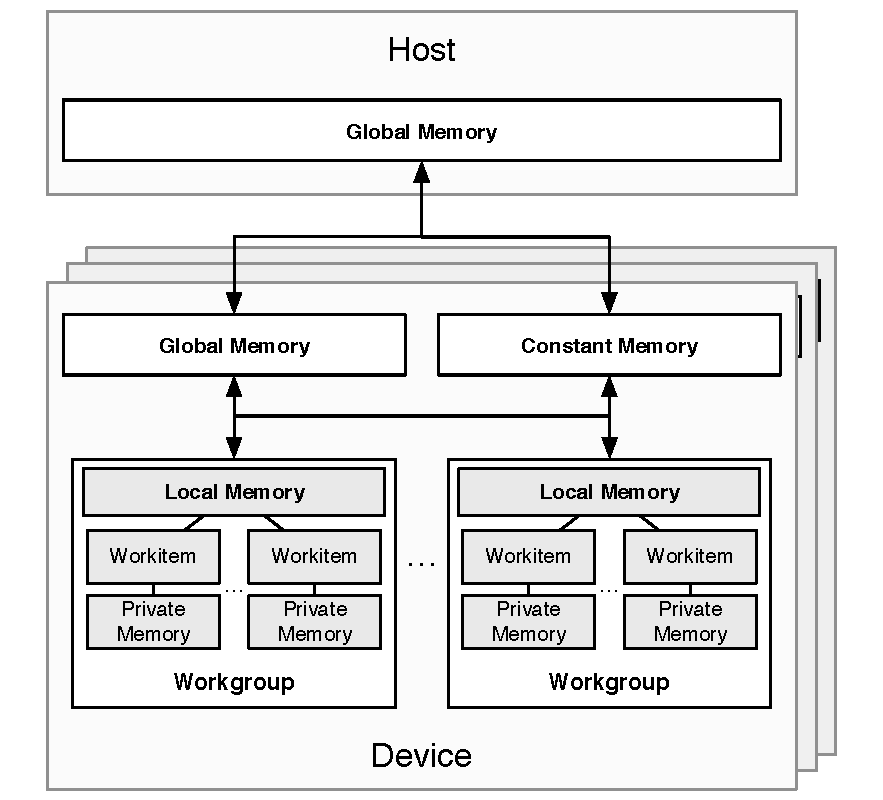
\includegraphics[width=0.8\textwidth]{img/opencl-memory}
	\caption[The OpenCL memory model]{%
		The OpenCL memory model. The host communicates with each device through transfers between global memory spaces. The capacity of each type of memory is dependent on the device hardware. In general, private memory is the fastest and smallest, and global memory is the largest and slowest.%
	}
	\label{fig:opencl-memory}
\end{figure}

\subsubsection{Performance Optimisations}

The wide range of supported execution devices and differing standards-compliant implementations makes portable performance tuning of OpenCL programs a difficult task~\cite{Rul2010}, and the interactions between optimisations and the hardware are complex and sometimes counter-intuitive~\cite{Ryoo2008}.

The overhead introduced by memory transfers between host and compute devices further complicates comparisons of OpenCL performance on different devices. The conclusion of~\cite{Gregg2011} is that this overhead can account for a $2\times$ to $50\times$ difference of GPU program runtime. In~\cite{Lee2010}, \citeauthor{Lee2010} present a performance analysis of optimised throughput computing applications for GPUs and CPUs. Of the 14 applications tested, they found GPU performance to be $0.7\times$ to $14.9\times$ that of multi-threaded CPU code, with an average of only 2.5$\times$. This is much lower than the $100\times$ to $1000\times$ values reported by other studies, a fact that they attribute to uneven comparison of optimised GPU code to unoptimised CPU code, or vice versa. \citeauthor{Lee2010} found that multi-threading, cache blocking, reordering of memory accesses and use of SIMD instructions to contribute most to CPU performance. For GPUs, the most effective optimisations are reducing synchronisation costs, and exploiting local shared memory. In all cases, the programs were optimised and hand-tuned by programmers with expert knowledge of the target architectures. It is unclear whether their performance results still hold for subsequent generations of devices.

Despite the concerns of over-represented speedups, the potential for high performance coupled with the complexity and low levels of abstraction provided by OpenCL make it an ideal target for skeletal abstractions. SkelCL and SkePU are two such examples which add a layer of abstraction above OpenCL and CUDA respectively in order to simplify GPGPU programming~\cite{Enmyren2010}.

\section{Summary}
\label{subsec:background-summary}
